\documentclass[a4paper]{article}

\usepackage[margin=2cm, right=2.3cm]{geometry}

\usepackage{fontspec}
\setmainfont{Liberation Serif}

\renewcommand\normalsize{\fontsize{12}{13.5}\selectfont}
\sloppy

\usepackage{tikz, pdfpages, luacode}

\begin{document}

\noindent
Задание 1. Выполнить п.7 на стр. 22 следующего методического указания: Аникин,
А. Ю. Ряды Фурье: метод. указания к выполнению типового расчета:
учебнометодическое пособие / А. Ю. Аникин, А. С. Савин, В. Я. Томашпольский. —
Москва: МГТУ им. Н.Э. Баумана, 2012. — 32 с. — URL:
https://e.lanbook.com/book/58442

\begin{tikzpicture}[remember picture, overlay]
  \node[yshift=-20pt] at (current page.center)
  {\includegraphics[
      page=22,
      width=22.5cm,
      clip,
      trim=0 90 0 160,
    ]{source}};
\end{tikzpicture}

\begin{luacode*}
function print_page(page_number)
  tex.print(string.format(
    [[\newpage]] ..
    [[\begin{tikzpicture}[remember picture, overlay] ]] ..
    [[\node[yshift=17mm] at (current page.center) {\includegraphics[ ]] ..
      [[page=%s, width=22.5cm, clip, trim=0 28mm 0 0, clip]{source}};]] ..
    [[\end{tikzpicture}]],
    page_number
  ))
end

for page_number=23,27 do
  print_page(page_number)
end
\end{luacode*}

\end{document}
